\documentclass[12pt,twoside,a4paper]{article} 
\usepackage{datetime}
\newdateformat{bkdate}{\THEYEAR-\shortmonthname-\twodigit{\THEDAY}}
\usepackage[pdftex]{graphicx}   
\usepackage{mathptmx}  
\DeclareGraphicsExtensions{.pdf,.jpeg,.png,.jpg}         
\usepackage{cite}
\usepackage{caption}
\usepackage{subcaption}

\begin{document}
    \pagenumbering{gobble}
    \begin{titlepage}
        \noindent
        Project: Smart Blossom
        \vspace{2em}
        \\
        {\fontsize{40}{50}\selectfont
        Development of \\[0.5em]
        a Blossom \\[0.5em]
        Shaped Lamp \\[0.5em]
        }
        \vspace*{\fill}
        \small 

        \hspace*{\fill} Written by \\
        \hspace*{\fill} Christopher Heiden \\
        \hspace*{\fill} MatNr.: 120249 \\
        \vspace{2em}

        \hspace*{\fill} Supervisor:  \\
        \hspace*{\fill} Wegener \\
        \vspace{2em}

        \hspace*{\fill} Submission: \\
        \hspace*{\fill} \bkdate\today
        
    \end{titlepage}
    \newpage

    \tableofcontents
    \newpage

    \pagenumbering{arabic}
    \setcounter{page}{3}

    \section{Introduction}
    \begin{flushleft}
        In a class called "Printed Interfaces", we try to create circuits that does not use common wires 
        to link sensors and microcontrollers. Therefore, we use conductive ink, conductive rubber or other
        material that can close a circuit, for example.\newline
    \end{flushleft}

    \section{Class Process}
    \begin{flushleft}
        To teach the class the major concepts of circuits and to create one with a microcontroller \footnote{\label{foot:microcontroller}Dies ist jetzt eine Fußnote.}, the 
        teacher taught the basic principles of Ohm's law, how the current flows and how to program a microcontroller.
        This has been done in the first 4 sessions.\newline
        In the first session, the teacher spoke about the current flow and Ohm's law. Therefore, he showed the students
        a virtual circuit that he could change in real-time.\newline
        In the second session, he talked about microcontrollers and how these devices can be used. He spent short
        time in explaining the pins and how to program them. To do so, he showed how it is possible to program
        everything on a projector (live coding). He showed us how to program an LED, simple moisture and 
        a capacitive sensor. The simple moisture and capacitive sensor has been drawn with conductive ink.\newline
        In the third lecture, he taught the students more about programming, so it became more complex. However, 
        the main focus was to introduce InkScape. With this program, we wanted to print a conductive circuit on paper.\newline
        Later he wanted us to find project ideas that we present. So, every student presented one or multiple ideas and
        the group talked about them. Sometimes, they discussed improvements and sometimes, they talk about the idea itself
        and the way to implement and build everything.
        Later we talked and discussed the projects more detailed, so anyone can start programming and building everything.
    \end{flushleft}

    \section{Project Process}
    \subsection{Ideas}
    \subsubsection{Color-changing Bracelet}
    \begin{flushleft}
        Our first idea was to program and color-changing bracelet. This can change its color if someone of your
        friends has such a bracelt too. These can create a network, so they can communicate with each other. The
        network strength can be used to identify if the friend is close. Then it will change its color, so both know
        that a friend is close to him or her. Also, groups can be defined. Every group has its own thread and if someone 
        from a specific group is next to you the system can change the color of this specific thread. This would just 
        be a proof of concept, so most of the programming would be static (see Figure ~\ref{fig:braceltIdea}).
    \end{flushleft}

    \begin{figure}[h!]
        \centering
        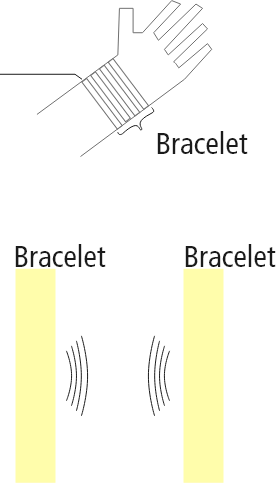
\includegraphics[scale=0.4]{images/projectideas/bracelt.png}
        \caption{Shows the bracelt concept.}
        \label{fig:braceltIdea}
    \end{figure}

    \subsubsection{Music controll Jacket}
    \begin{flushleft}
        Another idea was to develop a jacket that can be used to change a song you are listening on a phone. Therefore,
        strips are placed on the left or right arm that can be used to change the song to make it louder or to stop the song, 
        for example (see Figure ~\ref{fig:jacketIdea}).
    \end{flushleft}

    \begin{figure}[h!]
        \centering
        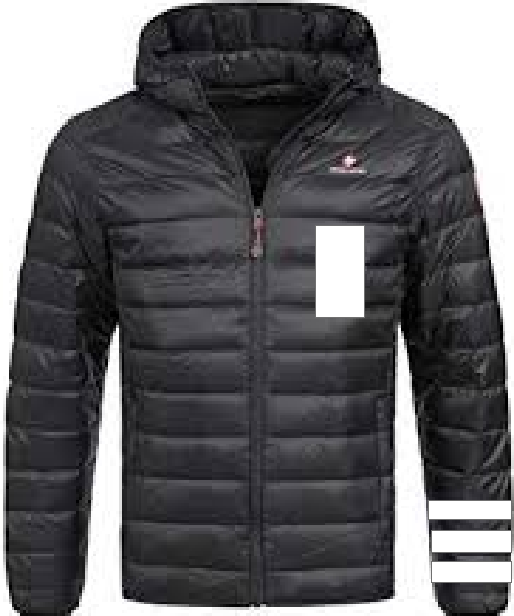
\includegraphics[scale=0.2]{images/projectideas/jacket.png}
        \caption{Shows the concept of a jacket with interaction constraints.}
        \label{fig:jacketIdea}
    \end{figure}

    %why is the new chapter before image? 
    \subsubsection{Blossom shaped Lamp}
    \label{BlossomShapedLamp}
    \begin{flushleft}
        A third and last idea is about lightness. The idea is to build a lamp of a blossom that can be modified by the user.
        Every blossom leaf has a magnet inside, so it is possible to connect each leave. If some leaves are connected, the lamp that 
        is in the middle of the flower blossom changes its color. Moreover, it is possible to rotate the whole lamp and to change the
        brightness by an analog switch (see Figure ~\ref{fig:blossomLamp}).
    \end{flushleft}

    \begin{figure}[h!]
        \centering
        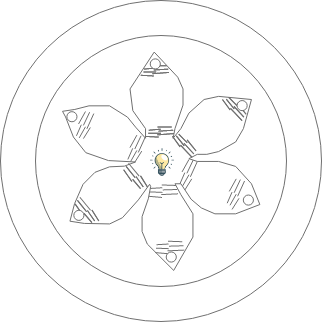
\includegraphics[scale=0.4]{images/projectideas/blossomLamp.png}
        \caption{Shows the concept of a blossom shaped lamp.}
        \label{fig:blossomLamp}
    \end{figure}

    \subsection{Detailed Idea}
        \begin{flushleft}
            At the end, we dicided to develop the third idea (see chapter \ref{BlossomShapedLamp}). That's why, we want to explain 
            how it should work in detail. \newline
            The base of the prototyp will be milled, so we get a perfect shape of the the base. Therefore, we will use Autodesk Fusion 360\cite{autodeskFusion360}
            to model it. in teh center of the base will be the blossom shaped lamp that can be opened. Around this, we want to have a 
            circled shaped groud. There we want to place cupper foil that is linked with a microcontroller, % add explaination
            so the foil ca be used as a slider. This interaction will change the brightness of the lamp. \newline
            However, the major functionality is the lamp itself. Therefore, we want to laser cut the shape, so the users of the lamp can
            take one or several blossoms to open it. This will change the color shining of the lamp. We want to use a transparent acrylic glass.
            Therfore, we have to cut holes inside the glass, so the shape can change.  \newline
            If all blossoms are connected, then the lamp doesn't shine at all. However, if the user open the blossom, then the lamp gets on
            and the color change. 
            \newline
            \newline
            To develop such a device, we want to use an Arduino Pro Mini, copper foil and programmable WS2812B leds.
            A three-dimensional model of the base can be found in Figure ~\ref{fig:blossomBaseModel}
            
            \begin{figure}[h!]
                \centering
                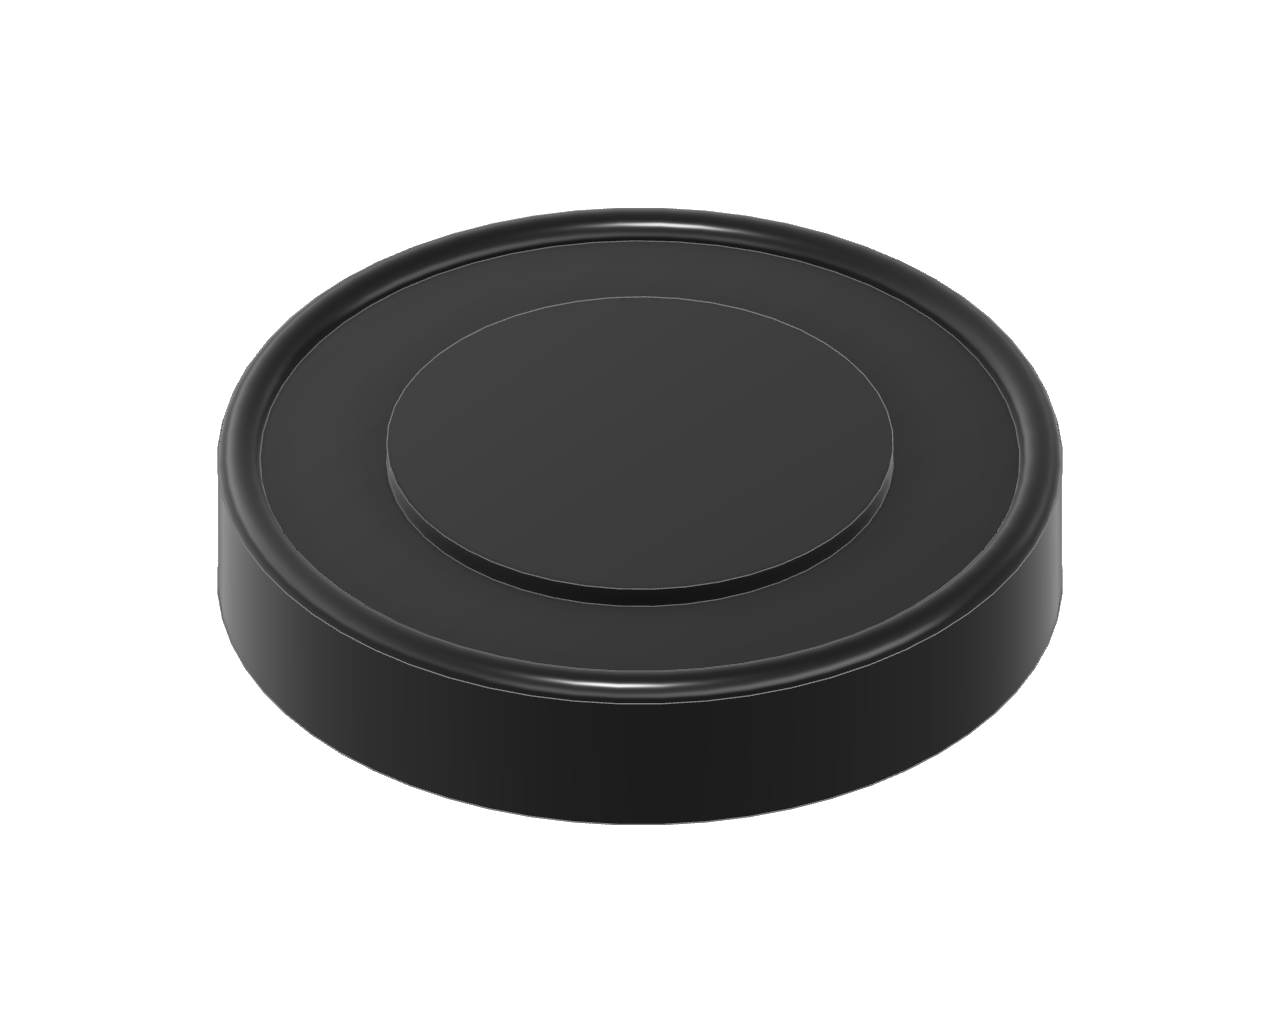
\includegraphics[scale=0.3]{images/process/FlowerLamp.png}
                \caption{Shows a three-dimensional base model of the blossom lamp idea.}
                \label{fig:blossomBaseModel}
            \end{figure}

        \end{flushleft}

    \subsection{Building Process}
        \begin{flushleft}
            To build the prototyp, we modeled the base for the lamp (see Figure ~\ref{fig:blossomBaseModel}). Therfore, we used
            Autodesk. After doing so, we used a milling machine. We only had to convert the 3D model into a .iges file.
            The result of the milling process can be seen in Figure ~\ref{fig:blossomBase}.
        \end{flushleft}

        \begin{figure}[h!]
            \centering
            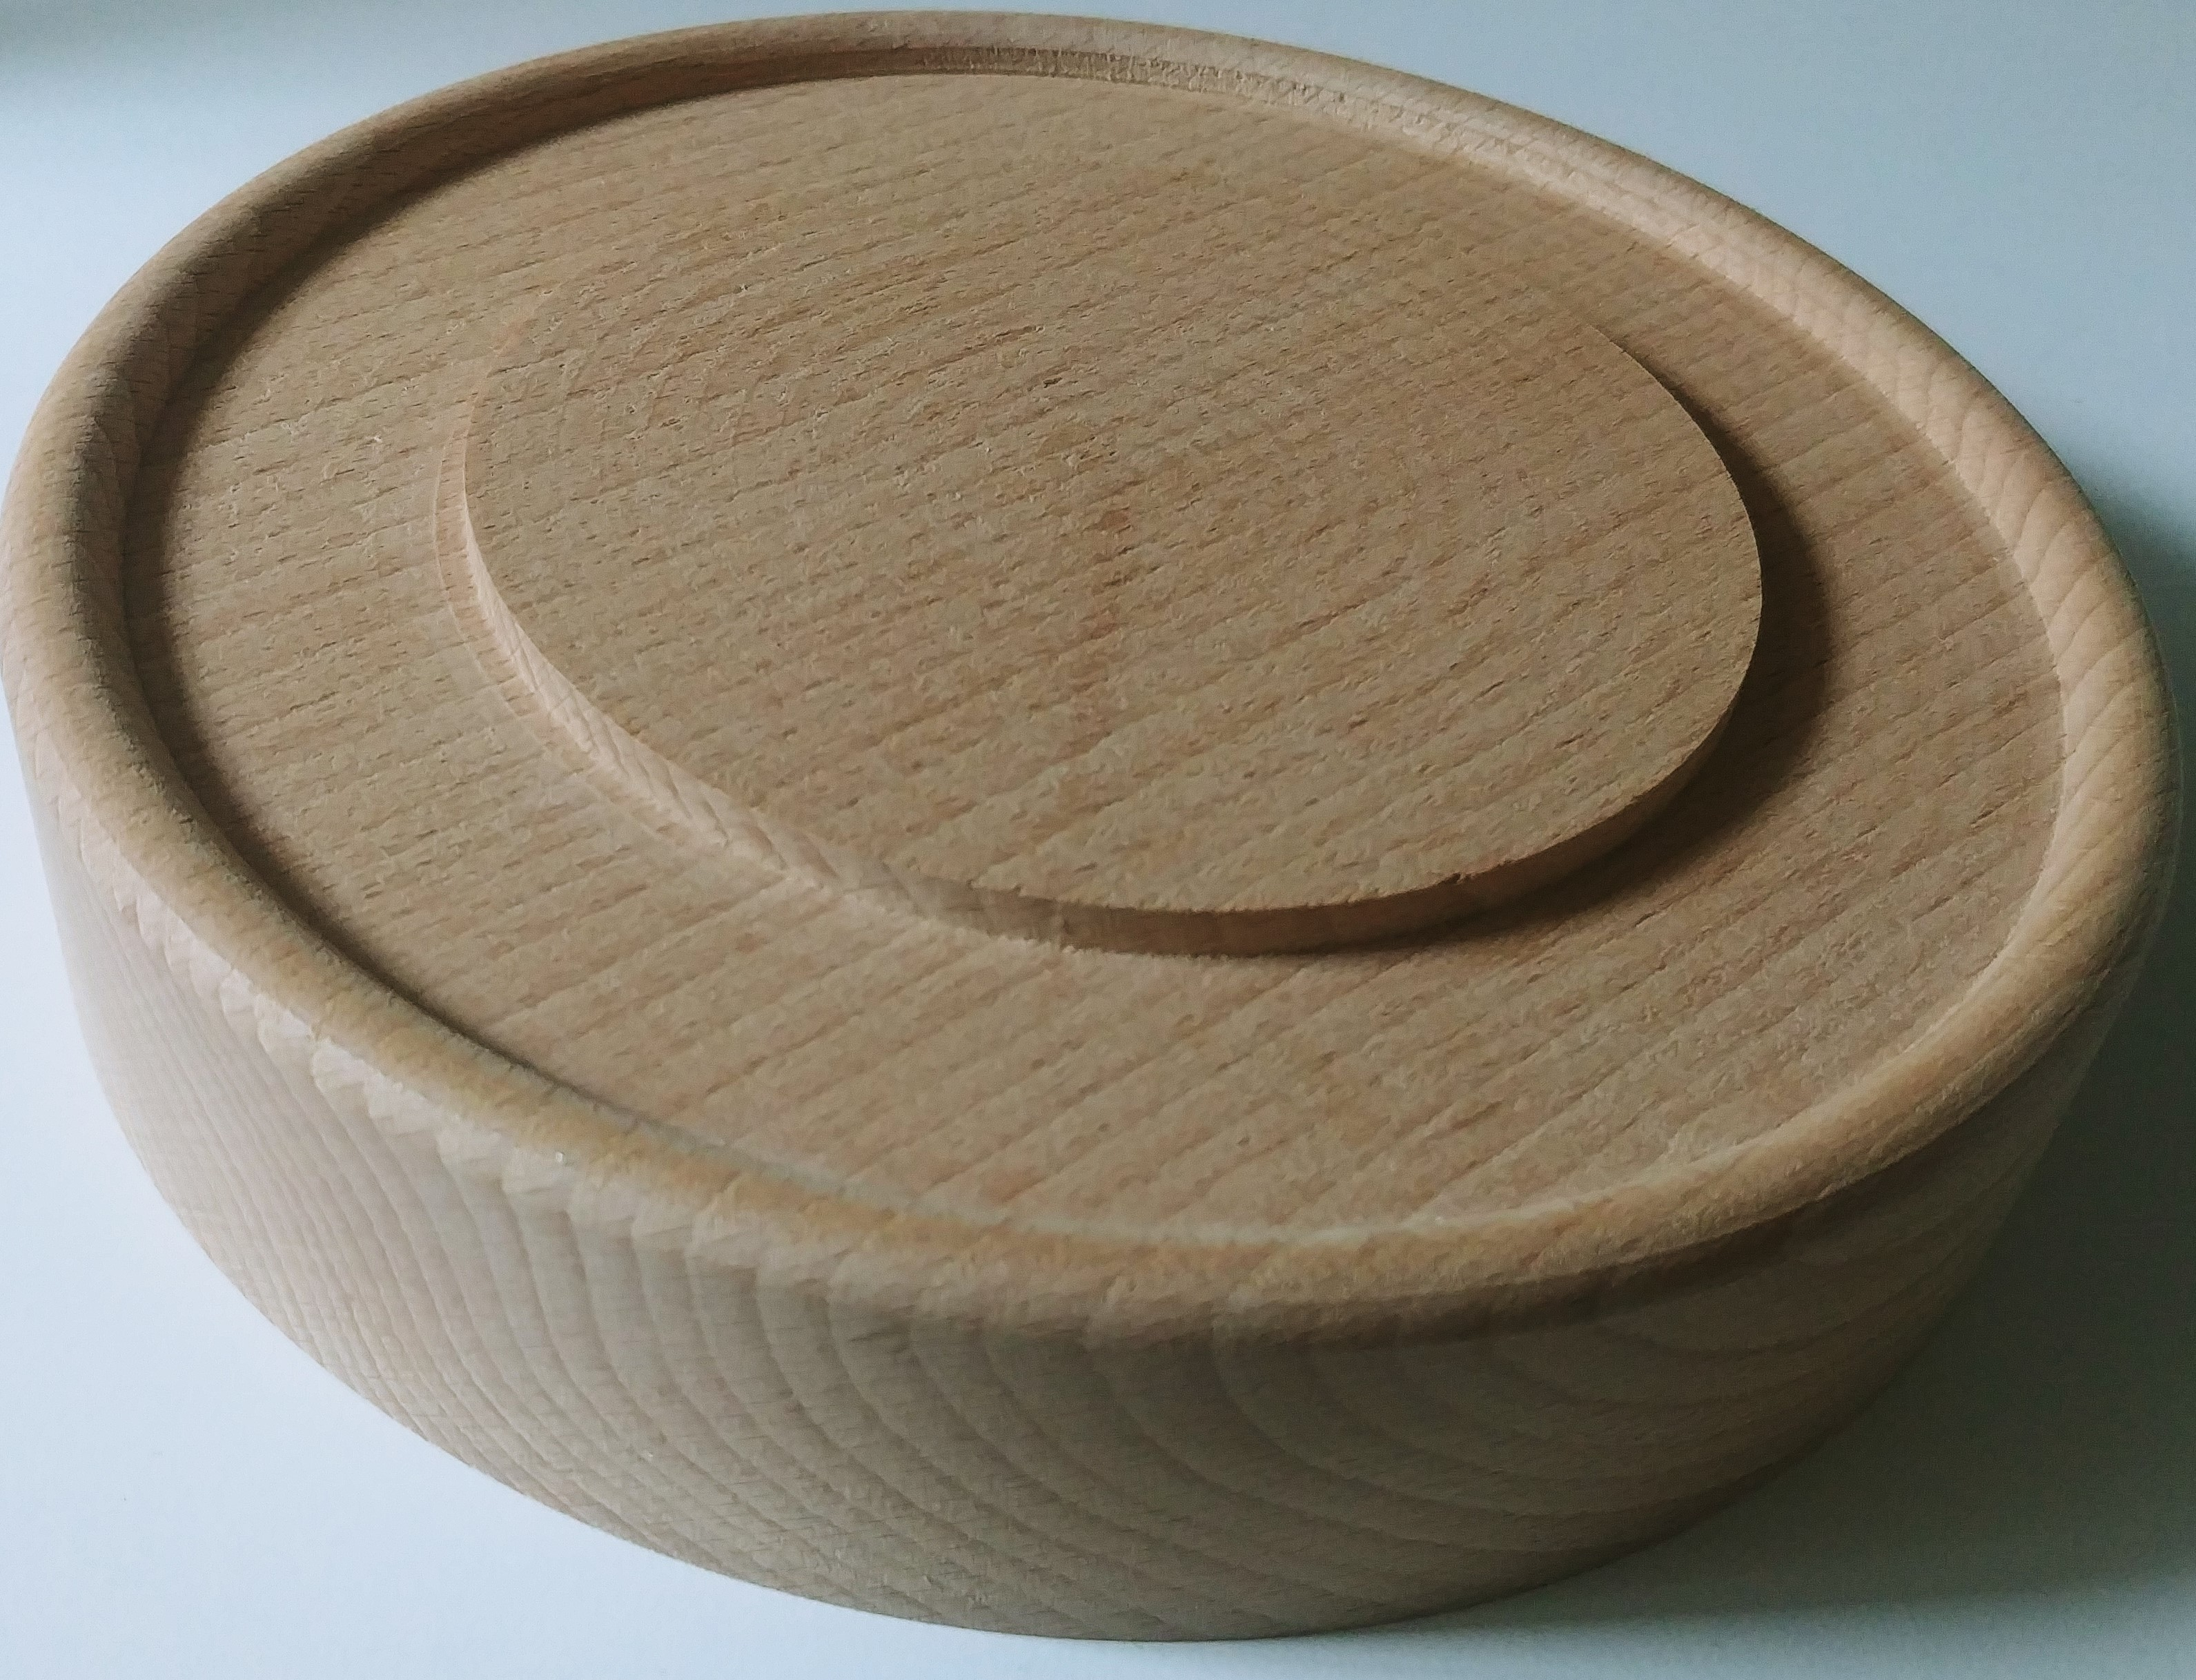
\includegraphics[scale=0.1]{images/process/base.jpg}
            \caption{Shows the base that has been milled.}
            \label{fig:blossomBase}
        \end{figure}

        After milling the base, we had to experiment with the lase cuter and how big the holes and the distance between them 
        should be, so we can laser cut the blossom shape later. To laser cut everything, we used Illustator\cite{illustrator} and a laser cutter. 
        With Illustator we can design the shape that has to be cut. Therfore, we tried a width of 1mm, 0.75mm and 0.5mm and a distance
        of 1mm, 0.75mm, 0.5mm. The result can be found in Figure ~\ref{fig:laserCutTests}.

        \begin{figure}[ht!]
            \centering
            \begin{subfigure}{.5\textwidth}
              \centering
              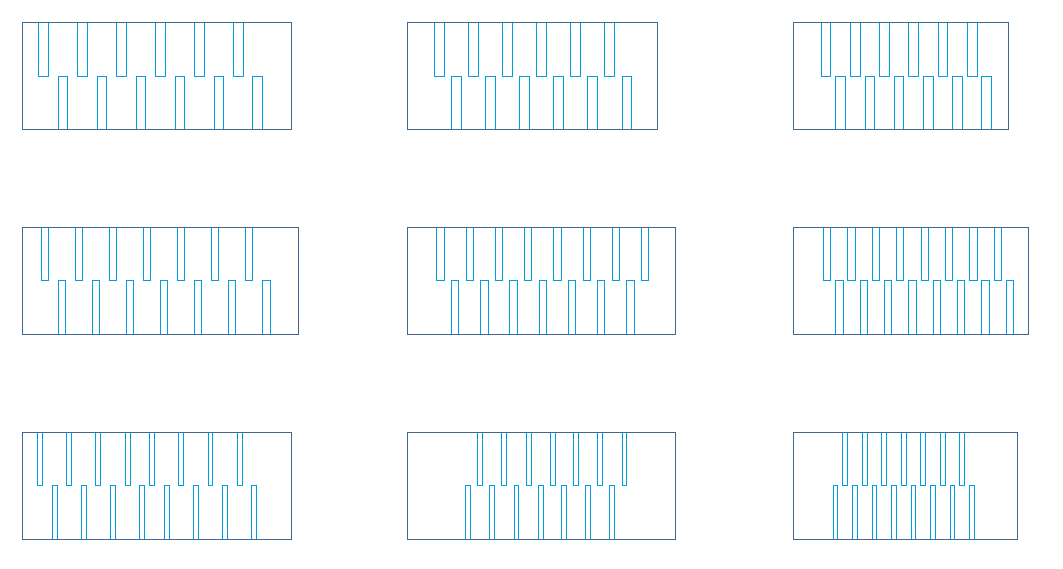
\includegraphics[width=.8\linewidth]{images/process/test_shapes.PNG}
              \caption{Shows the test shapes from Illustator.}
              \label{fig:test_shapes}
            \end{subfigure}%
            \begin{subfigure}{.5\textwidth}
              \centering
              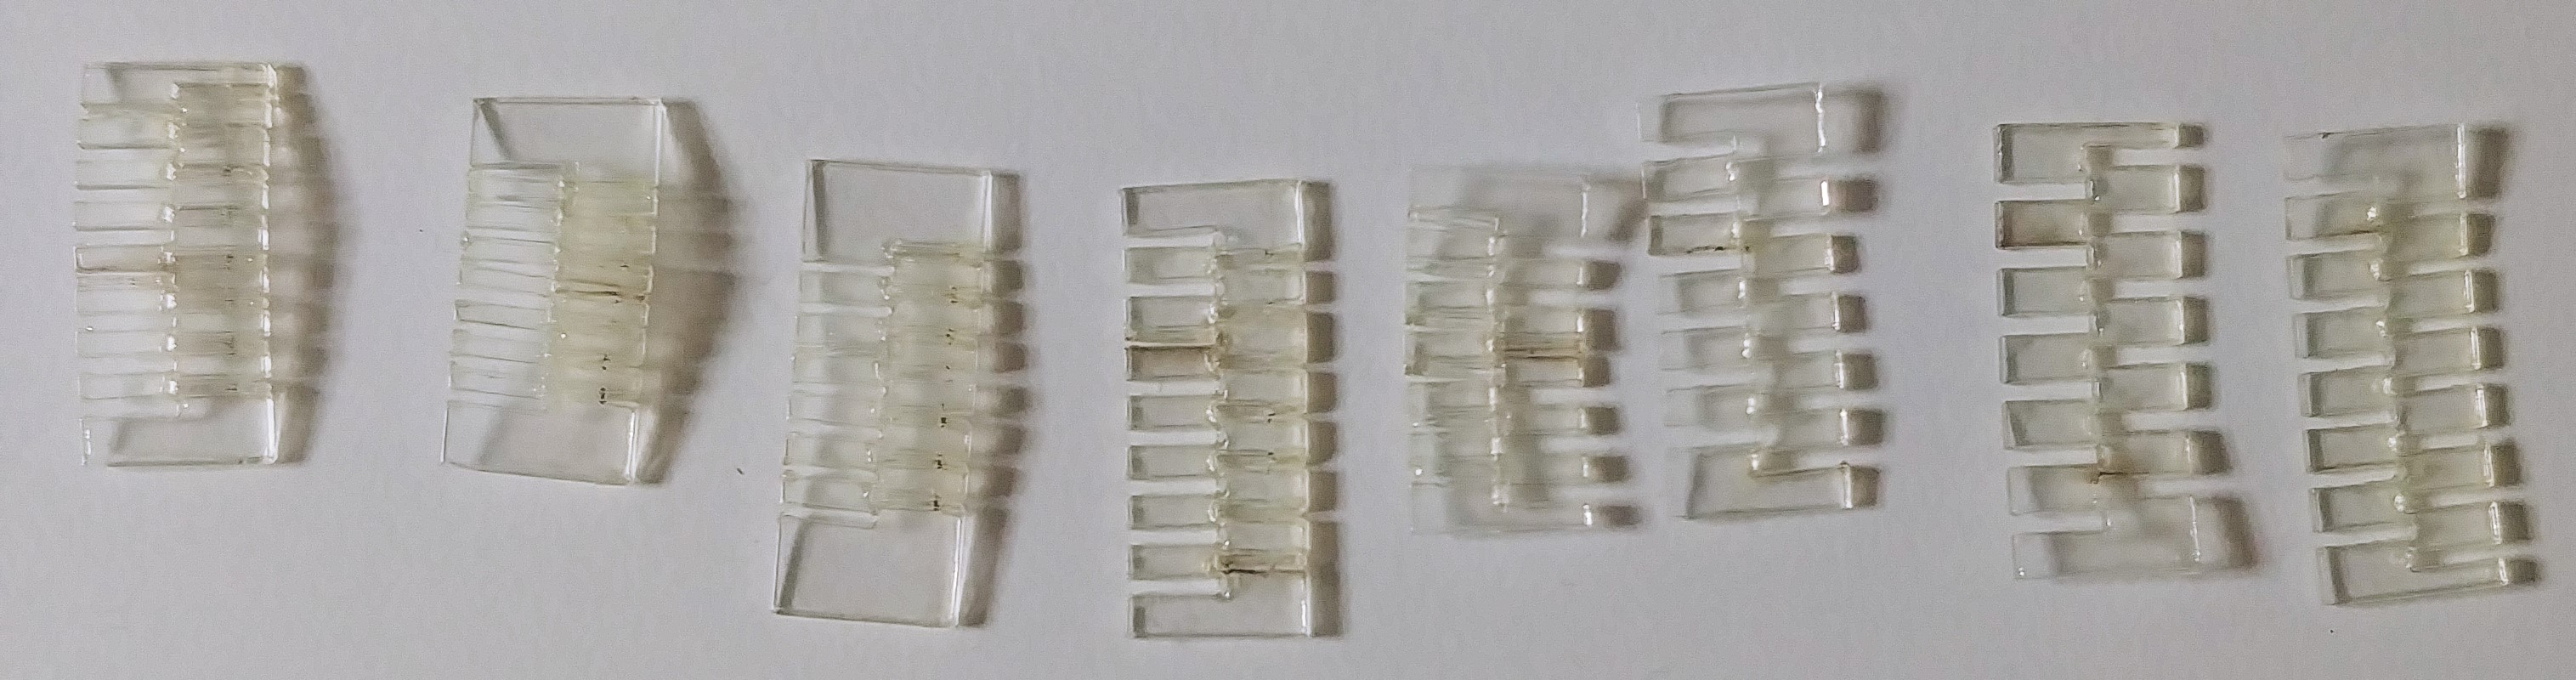
\includegraphics[width=.8\linewidth]{images/process/laserCutTests.jpg}
              \caption{Shows the laser cutted tests.}
              \label{fig:ringdesign2}
            \end{subfigure}
            \caption{Shows ring design.}
            \label{fig:laserCutTests}
        \end{figure}

        Afterwards, we could laser cut the blossom.
        
        % has to be changed later
        \begin{figure}[ht!]
            \centering
            \begin{subfigure}{.5\textwidth}
              \centering
              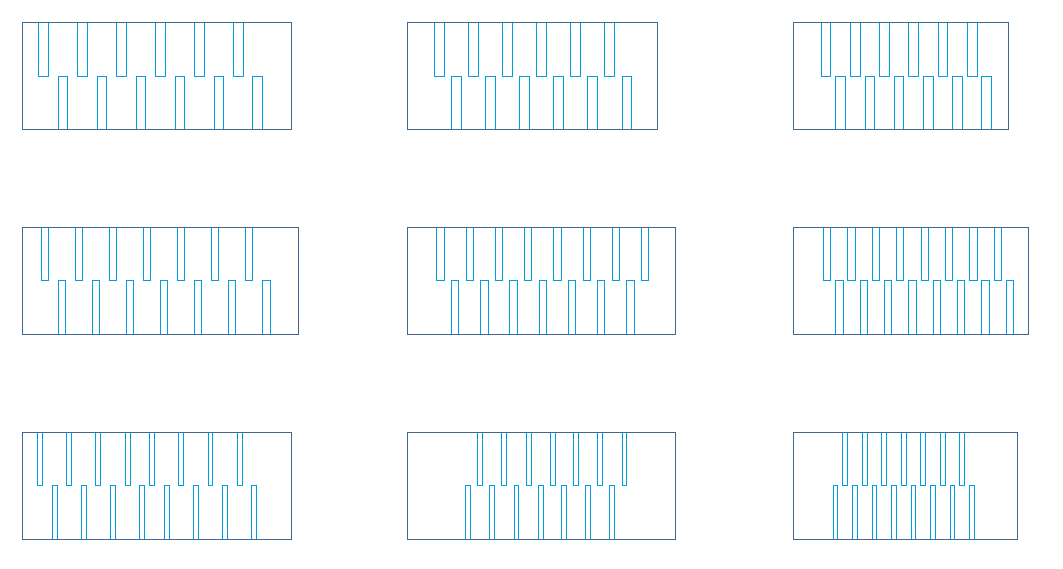
\includegraphics[width=.8\linewidth]{images/process/test_shapes.PNG}
              \caption{Shows the laser cutted tests.}
              \label{fig:test_shapes}
            \end{subfigure}%
            \begin{subfigure}{.5\textwidth}
              \centering
              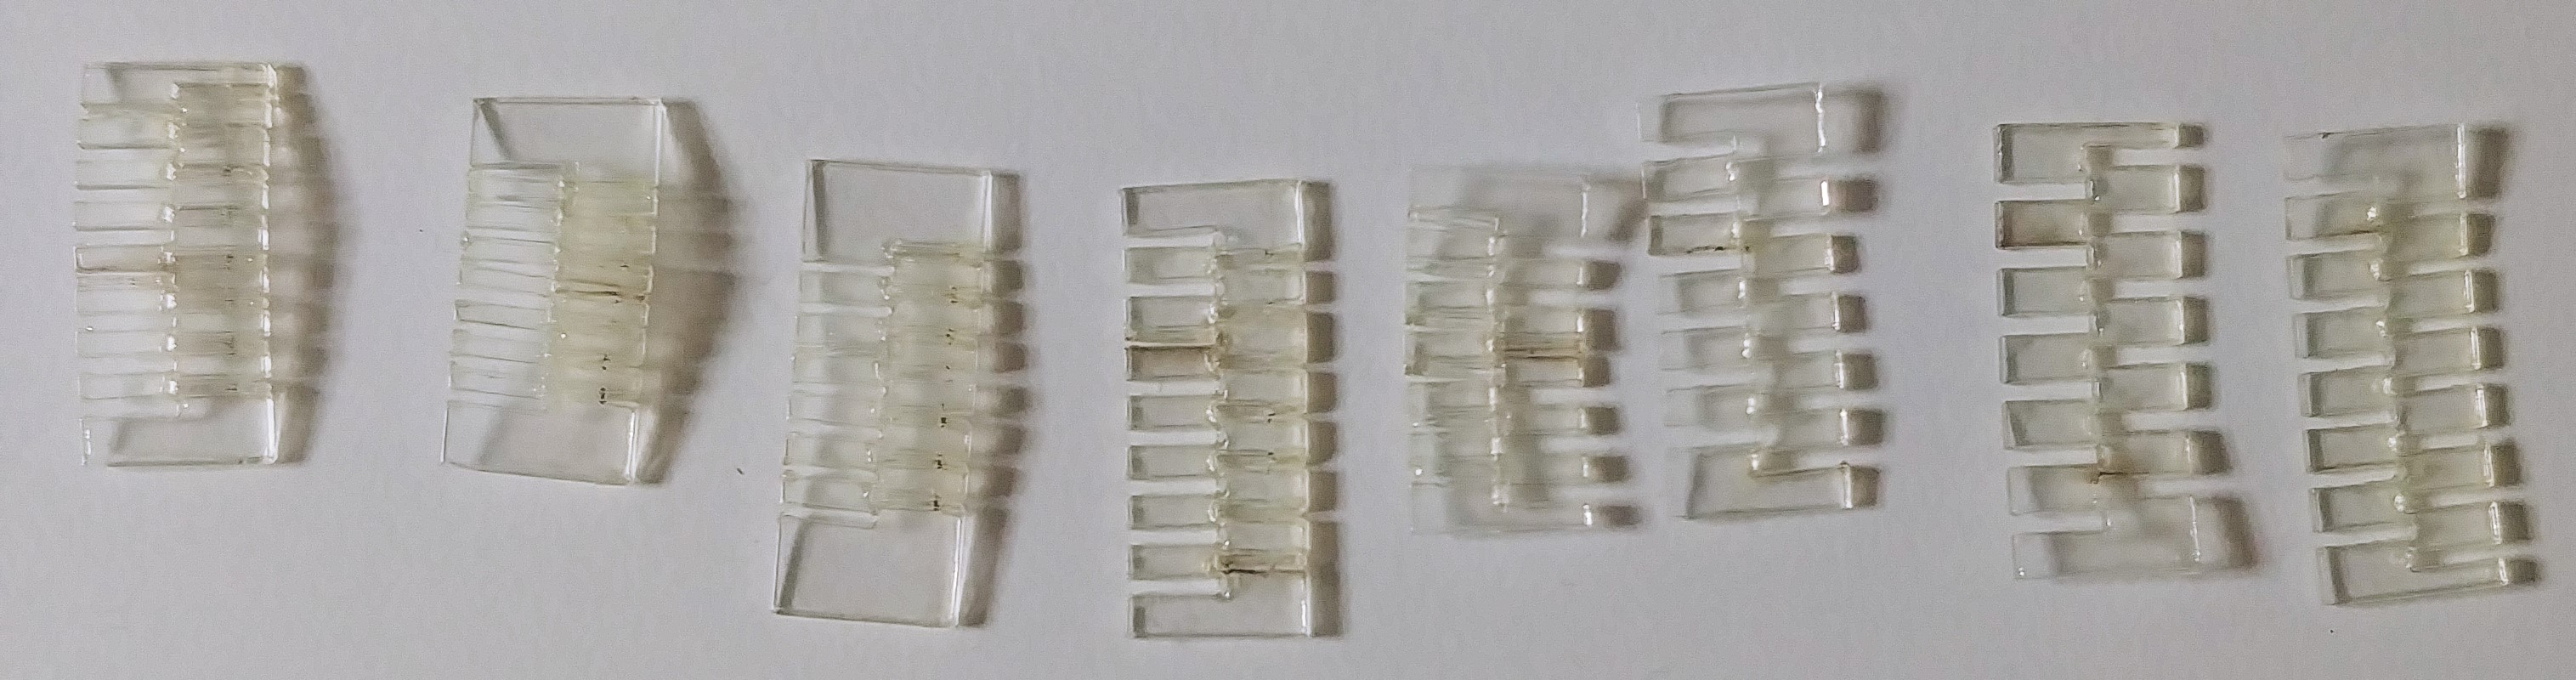
\includegraphics[width=.8\linewidth]{images/process/laserCutTests.jpg}
              \caption{Shows the laser cutted tests.}
              \label{fig:ringdesign2}
            \end{subfigure}
            \caption{Shows ring design.}
            \label{fig:laserCutTests}
        \end{figure}

    \subsection{Implementation}
        \begin{flushleft}
        dwadwad
        \end{flushleft}

    \subsubsection{Coding the LED strip}
        \begin{flushleft}
        dwadwa
        \end{flushleft}

    \subsubsection{Coding the slider}
        \begin{flushleft}
        das ist ein test text (see Table ~\ref{tab:test}).\newline
        \end{flushleft}

        \begin{table}[h]
            \centering
            \begin{tabular}[h]{ccc}
                & Code &  \\
                & Show Code &  \\
            \end{tabular}
            \caption{Shows the con}
            \label{tab:test}
        \end{table}
        \begin{flushleft}
        \end{flushleft}


    \subsubsection{Merging code and physical components}
        \begin{flushleft}
        \end{flushleft}

    \section{Outcome}
        \begin{flushleft}

            The code can be found on GitHub: 
        \end{flushleft}
        
    \newpage
    \bibliography{assignment_3} 
    \bibliographystyle{ieeetr}

    \newpage
    \section{Annex}

        \begin{tabular}[h]{ccc}
            & Code &  \\
            & Show Code &  \\
        \end{tabular}
\end{document}